\documentclass[a4paper,12pt]{article}
\usepackage[T1]{fontenc}
\usepackage[utf8]{inputenc}
\usepackage[polish]{babel}
\let\lll\undefined
\usepackage{amssymb}
\usepackage{amsthm}
\usepackage{graphicx}
\usepackage{times}
\usepackage{anysize}

\marginsize{1.5cm}{1.5cm}{1.5cm}{1.5cm}
\sloppy 

\theoremstyle{definition}
\newtheorem{df}{Definicja}


\begin{document}

% \mathbf

\section*{Całka Riemanna}
Niech dana będzie funkcja ograniczona $ f \colon [a,b] \rightarrow \mathbb{R}$. \textit{\textsf{Sumą częściową}} (Riemanna) nazywa się liczbę
$${R_{f,P(q_{1},\dots ,q_{n})}=\sum _{i=1}^{n}f(q_{i})\cdot \Delta p_{i}.}$$
Funkcję $f$ nazywa się \textit{\textsf{całkowalną w sensie Riemanna}} lub krótko \textit{\textsf{R-całkowalną}}, jeśli dla dowolnego ciągu normalnego $ (P^{k})$ podziałów przedziału $[a,b]$, istnieje (niezależna od wyboru punktów pośrednich) granica
$$
	R_f = \lim_{k \to \infty} R_{f,P^k(q_1^k , \dots , q_{n_k}^k)}
$$
nazywana wtedy \textbf{\textsf{całką Riemanna}} tej funkcji. Równoważnie: jeżeli istnieje taka liczba $R_{f},$  że dla dowolnej liczby rzeczywistej $ \varepsilon >0$  istnieje taka liczba rzeczywista $\delta >0,$ że dla dowolnego podziału $ P(q_{1},\dots ,q_{n})$ o średnicy $ \mathrm {diam} \;P(q_{1},\dots ,q_{n})<\delta ;$ bądź też w języku rozdrobnień: że dla dowolnej liczby rzeczywistej $ S(t_{1},\dots ,t_{m})$ przedziału$[a,b]$, że dla każdego podziału $ P(q_{1},\dots ,q_{n})$ rozdrabniającego $ S(t_{1},\dots ,t_{m})$ zachodzi
$$ \left|R_{f,P(q_{1},\dots ,q_{n})}-R_{f}\right|<\varepsilon . $$
Funkcję $f$ nazywa się wtedy całkowalną w \textit{\textsf{sensie Riemanna (R-całkowalną)}}, a liczbę $R_{f}$ jej \textbf{\textsf{całką Riemanna}}.

\begin{figure}[!htb]
	\centerline{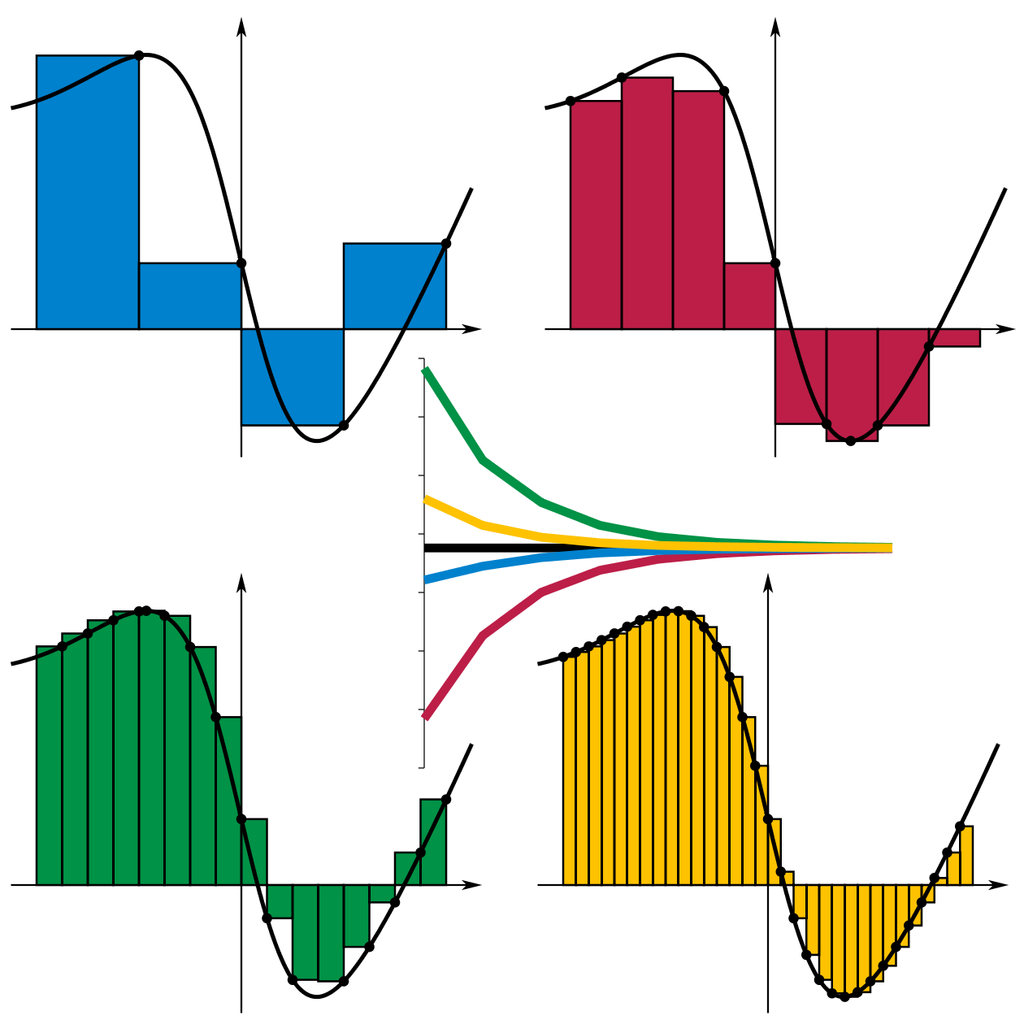
\includegraphics{przykladSum}}
	\caption{Przykład sum Riemanna przy wyborze punktu pośredniego w prawym końcu podprzedziału (niebieski), w wartości minimalnej (czerwony) i maksymalnej (zielony) funkcji w podprzedziale i lewego końca podprzedziału (żółty). Wartość wszystkich czterech przypadków zbliża się do 3,76 przy powiększaniu liczby podprzedziałów od 2 do 10 (w domyśle, również nieograniczenie).}
	\label{fig:Przyklad sum}
\end{figure}


\end{document}
